\section*{Exercice 1}
\setcounter{subparagraph}{0}

Soit l'algorithme suivant : 

\begin{py}
\begin{python}
def mult(n, p):
    if p == 0:
        return 0
    else :
        return n+mult(n,p-1)
\end{python}
\end{py}

\subparagraph{}
\textit{Énoncer un variant de boucle et montrer la terminaison de l'algorithme.}

\subparagraph{}
\textit{Énoncer un invariant de boucle et montrer la correction de l'algorithme.}
\ifprof
\begin{corrige}
\begin{itemize}
\item Soit $\mathcal{P}$ la propriété d'invariance: à l'itération $p$, on a $mult(n,p)=n\cdot p$. 
\item À l'instant 0, on a : d'une part : $\forall n$, $n\cdot 0 = 0$. D'autre part, \texttt{mult(n,0)} renvoie 0. La propriété de récurrence est vraie. 
\item À l'instant $p$, on considère la propriété de récurrence est vraie à l'instant $p$ : $mult(n,p)=n\cdot p$.
\item À l'instant $p+1$, on applique l'algorithme : $p$ étant différent de 0, l'algorithme retourne $mult(n,p+1)=n+mult(n,p)$. D'après la propriété de récurrence, on a donc $mult(n,p+1)=n+ n\cdot p =n(p+1) $. La propriété est donc vraie au rang $p+1$.
\item L'algorithme calcule donc le produit $np$.
\end{itemize}
\end{corrige}
\else
\fi

\subparagraph{}
\textit{Donner et justifier la complexité temporelle de la fonction \texttt{mult}.}
\ifprof
\begin{corrige}
On note $C(p)$ le nombre d'appels récursifs : $C(p) = 1+C(p-1) = 1+1+C(p-2)=p+T(0)$. On a donc $C(p)=\mathcal{O}(p)$. La complexité temporelle est linéaire.
\end{corrige}
\else
\fi

\subparagraph{}
\textit{Donner et justifier la complexité spatiale de la fonction \texttt{mult}.}
\ifprof
\begin{corrige}
On stocke une valeur à chaque appel récursif. Si ce stockage est à coût constant, étant donné qu'il y a $n$ appels récursifs, la complexité spatiale est en $\mathcal{O}(n)$.
\end{corrige}
\else
\fi

\section*{Exercice 2}
\setcounter{subparagraph}{0}

Soit l'algorithme suivant : 

\begin{py}
\begin{python}
def puiss(x, n):
    if n == 0:
        return 1
    else :
        return x*puiss(x,n-1)
\end{python}
\end{py}

\subparagraph{}
\textit{Énoncer un variant de boucle et montrer la terminaison de l'algorithme.}

\subparagraph{}
\textit{Énoncer un invariant de boucle et montrer la correction de l'algorithme.}
\ifprof
\begin{corrige}
\begin{itemize}
\item Soit $\mathcal{P}$ la propriété d'invariance: à l'itération $p$, on a $puiss(x,n)=x^n$. 
\item À l'instant 0, on a : d'une part : $\forall x>0$, $x^0 = 1$. D'autre part, \texttt{puiss(x,0)} renvoie 1. La 
propriété de récurrence est vraie. 
\item À l'instant $n$, on considère la propriété de récurrence est vraie et à l'instant $p$ : $puiss(x,n)=x^n$.
\item À l'instant $n+1$, on applique l'algorithme : $n$ étant différent de 0, l'algorithme retourne 
$puiss(x,n+1)=x*mult(x,n)$. D'après la propriété de récurrence, on a donc $puiss(x,n+1)=x*x^n=x^{n+1} $. La propriété 
est donc vraie au rang $n+1$.
\item L'algorithme calcule donc le produit $x^n$.
\end{itemize}   
\end{corrige}
\else
\fi
\subparagraph{}
\textit{Donner et justifier la complexité temporelle de la fonction \texttt{puiss}.}
\ifprof
\begin{corrige}
On note $C(p)$ le nombre d'appels récursifs : $C(p) = 1+C(p-1) = 1+1+C(p-2)=p+T(0)$. On a donc $C(p)=\mathcal{O}(p)$. La 
complexité temporelle est linéaire.
\end{corrige}
\else
\fi

\subparagraph{}
\textit{Donner et justifier la complexité spatiale de la fonction \texttt{puiss}.}
\ifprof
\begin{corrige}
On stocke une valeur à chaque appel récursif. Si ce stockage est à coût constant, étant donné qu'il y a $n$ appels 
récursifs, la complexité spatiale est en $\mathcal{O}(n)$.
\end{corrige}
\else
\fi



\section*{Exercice 3}
\setcounter{subparagraph}{0}

Soit l'algorithme suivant : 

\begin{py}
\begin{python}
def rechecheDichoRec(x, l):
    n=len(l)
    if n == 0:
        return False
    elif x<l[n//2] :
        return rechecheDichoRec(x, l[0:n//2])
    elif :
        return rechecheDichoRec(x, l[n//2:n])
    else :
        return True
\end{python}
\end{py}

\subparagraph{}
\textit{Donner et justifier la complexité temporelle de la fonction \texttt{rechecheDichoRec}.}
\ifprof
\begin{corrige}
Définissons le coût temporel comme le nombre d'appel récursif. Dans le pire des cas, l'élément n'est pas dans la liste. 
 On cherche $p$ le nombre de fois que $n$ est divisible par 2. On cherche donc $p$ tel que 
$n\left(\dfrac{1}{2}\right)^p>1 \Leftrightarrow p\ln \left(\dfrac{1}{2}\right)>\ln\left(\dfrac{1}{n}\right) 
\Leftrightarrow  p>\dfrac{\ln\left(\dfrac{1}{n}\right)}{\ln\left(\dfrac{1}{2}\right)} 
=\dfrac{-\ln\left(n\right)}{-\ln\left(2 \right)}   =\dfrac{\ln\left(n\right)}{\ln\left(2 \right)}$. La complexité est 
logarithmique. 
\end{corrige}
\else
\fi

\subparagraph{}
\textit{Donner et justifier la complexité spatiale de la fonction \texttt{rechecheDichoRec}.}
\ifprof
\begin{corrige}
On stocke une liste à chaque appel récursif. On note $n$ le coût de stockage d'une liste de taille $n$. Soit une liste 
\texttt{l} de taille $n=2^k$ avec $k\in \mathbb{N}$. 
À chaque itération, on stocke une liste de taille $n/2$.
On a donc $C(n)=n+\dfrac{n}{2}+\dfrac{n}{4}+...+1$. 

Par conséquent, $C(n)=2^k+\dfrac{2^k}{2}+\dfrac{2^k}{4}+...+1=2^k+2^{k-1}+2^{k-2}+...+1$. S'agissant de la somme des 
termes d'une suite géométrique :
$C(n)=1+2^1+...+2^k =\dfrac{1-2^{k+1}}{1-2} =2n+1$. La complexité spatiale est donc linéaire. 
\end{corrige}
\else
\fi


\section*{Exercice 4 -- Flocon de Von Koch}
\setcounter{subparagraph}{0}


Dans cet exercice, vous utiliserez des tableaux \textbf{numpy} pour représenter les points. C'est plus pratique que les 
listes python pour faire les calculs vectoriels.

\begin{itemize}
\item Si $a$ et $b$ représentent respectivement les points $(x,y)$ et $(x',y')$ alors $a+b$ représente le point 
$(x+x',y+y')$.
\item Si $r$ est un réel et $a$ représente le point de coordonnées $(x,y)$ alors $r*a$ représente le point $(rx,ry)$.
\item Si $a$ et $b$ sont des tableaux \textbf{numpy} alors $dot(a,b)$ représente le produit matriciel $a\times b$ (si ce 
produit est possible). La fonction \textbf{dot} est une fonction \textbf{numpy}.
\end{itemize}

Le mathématicien suédois Von Koch a défini la courbe du même nom dont voici les premières itérations.

\begin{center}
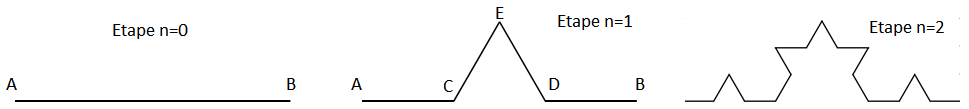
\includegraphics[width=.95\linewidth]{images/etapes_flocon}
\end{center}

\subparagraph{}
\textit{Ecrire une fonction \texttt{rotation} d'argument un réel \texttt{alpha} qui renvoie le tableau \textbf{numpy} 
correspondant à la matrice de rotation d'angle \texttt{alpha}.}

\subparagraph{}
\textit{Pour l'étape $n=1$, exprimer les points $C$ et $D$ en fonction de $A$ et $B$.}
En utilisant une matrice de rotation, exprimer $E$ en fonction de $C$ et $D$.

\subparagraph{}
\textit{En déduire une fonction récursive \texttt{koch} d'arguments les points \texttt{A} et \texttt{B} et un entier 
\texttt{n}. Cette fonction tracera la courbe de Von Koch pour l'itération $n$ à partir des points $A$ et $B$.}

\subparagraph{}
\textit{Ecrire une fonction \texttt{flocon} d'arguments les points $A$ et $B$ et un entier $n$. Cette fonction tracera 
le flocon de Von Koch pour l'itération $n$ à partir des points $A$ et $B$.}

\begin{center}
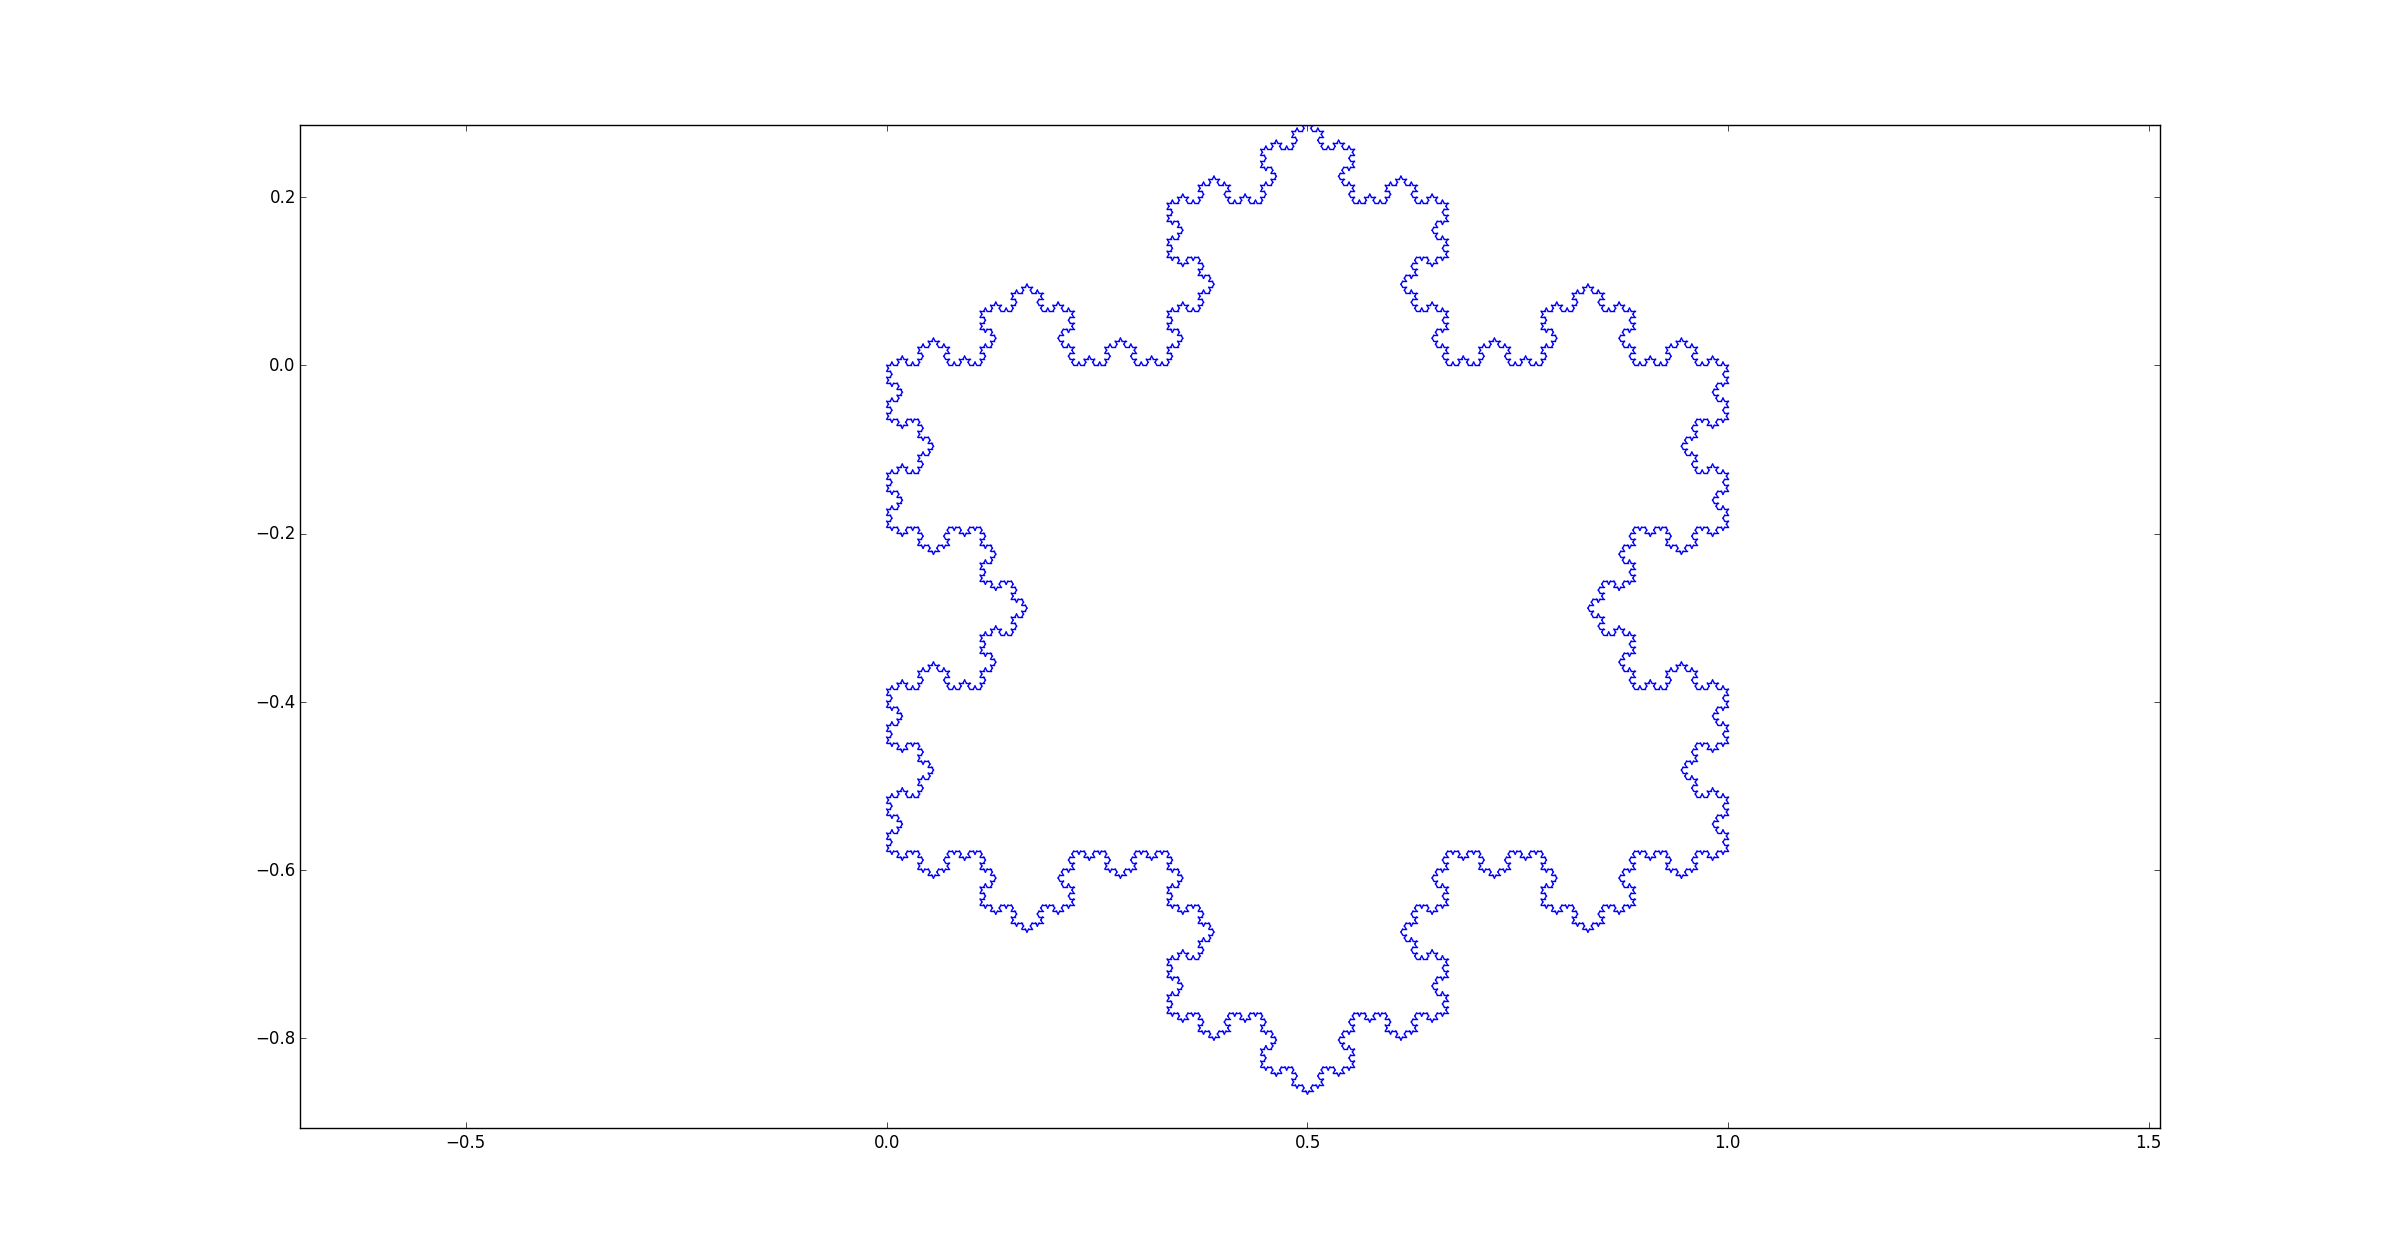
\includegraphics[width=.95\linewidth]{images/flocon_von_koch}
\end{center}

\ifprof
\begin{corrige}
\begin{python}
#matrice rotation d'angle pi/3
def rotation(angle):
    return np.array([[np.cos(angle),-np.sin(angle)],[np.sin(angle),np.cos(angle)]])

# angle=np.pi/3    
# print (rotation(angle))

def koch(a, b, n):
    R = rotation(np.pi/3)
    if n == 0:
        plt.plot([a[0], b[0]], [a[1], b[1]],'b')
    else:
        c=np.array([(b[0]-a[0])/3+a[0],(b[1]-a[1])/3+a[1]])
        d=np.array([2*(b[0]-a[0])/3+a[0],2*(b[1]-a[1])/3+a[1]])
        vecteur=d-c
        e=np.dot(rotation(np.pi/3),vecteur)+c
        koch(a, c, n - 1)
        koch(c, e, n - 1)
        koch(e, d, n - 1)
        koch(d, b, n - 1)
        
def flocon(a,b,n):
    koch(a,b,n)
    vecteur=b-a
    c=np.dot(rotation(-2*np.pi/3),vecteur)+b
    koch(b,c,n)
    koch(c,a,n)

n = 5
a = np.array([0,0])
b = np.array([1,0])
flocon(a, b, n)
plt.axis('equal')
plt.show()
\end{python}
\end{corrige}
\else
\fi

